\section{Result and discussion}%
\label{sec:result_and_discussion}

The resulting product is an open-source temperature monitoring system suitable for beer fermentation. The user of the web application can filter through time-series data by filtering the start and end date using callback functions that communicates with the database. In order to set an alarm level for detecting a temperature drop, these callback functions are also used to write a non-volatile setting to the database. This is helping the brewer to avoid oxidation through the airlock caused by back pressure.
Standard features provided by the Plotly library lets the user zoom and mouse-hover above the data points in order to receive immediate information about the temperature reading. 

\begin{figure}[h]
  \centering
  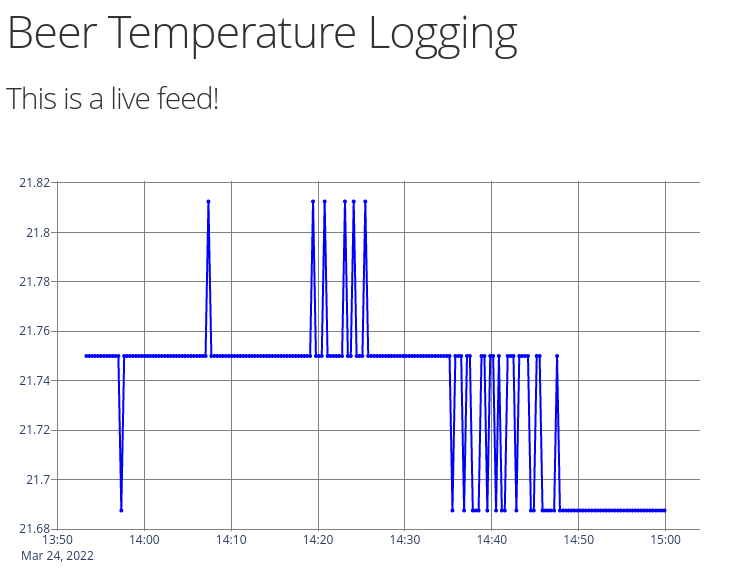
\includegraphics[width=0.8\textwidth]{/home/auan/Project/Report/Images/dash2.png}
  \caption{Live data graphed in Plotly Dash}
  \label{fig:dash2}
\end{figure}

The first part of the website grid is a live data feed that is shows the wanted amount of the latest data in Listing \ref{fig:dash2}.
\newpage

\begin{figure}[h]
  \centering
  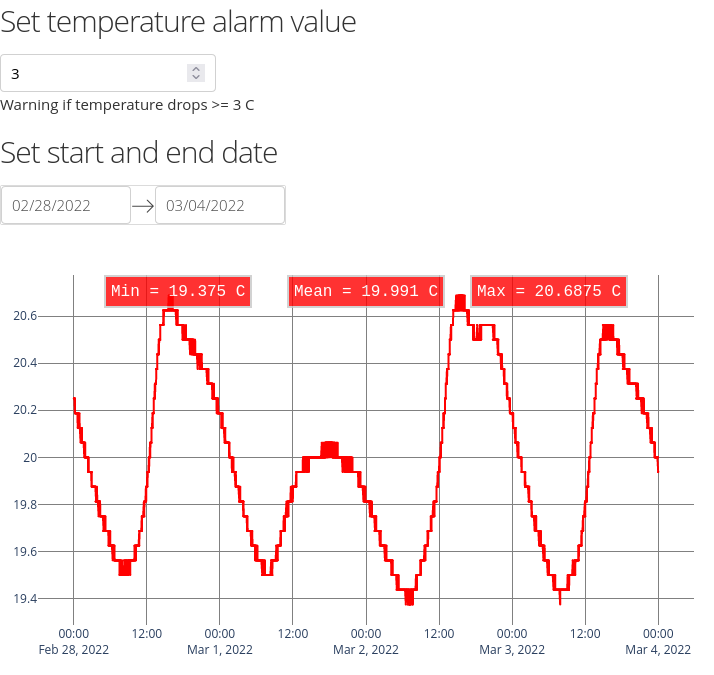
\includegraphics[width=0.7\textwidth]{/home/auan/Project/Report/Images/dash1.png}
  \caption{The time series temperature data graphed in Plotly Dash}
  \label{fig:dash1}
\end{figure}

In Figure \ref{fig:dash2}, the date picker above the graph gets the first and last dates of the time series. It handles input exceptions and only accept values in that specified range. The temperature drop alert puts the value in the database and is ready to send the alert if the next temperature reading triggers the alarm.

Viewing the unfiltered data points gives an overall view of the temperature fluctuations during longer time spans. When viewing in smaller time windows, the signal is in need of filtering by the MCU to reduce noise and provide a smoother curve.

\begin{lstlisting}[language=c, caption = {Logging entries in the Linux Journal as a result of the running system}, label = {lst:journal}]
Mar 16 06:27:42 alarm systemd[359]: Starting Reads serially from /dev/ttyUSB0 and puts in MongoDB...
Mar 16 06:27:49 alarm python[18967]: Running tests on port: /dev/ttyUSB0
Mar 16 06:27:49 alarm python[18967]: Baud rate = 9600
Mar 16 06:27:50 alarm python[18967]: Correct reading: 19.9375
Mar 16 06:27:50 alarm python[18967]: Correct reading: 19.9375
Mar 16 06:27:51 alarm python[18967]: Correct reading: 19.4375
Mar 16 06:27:51 alarm python[18967]: Passed init tests on 3 correct readings and 0 faulty readings
Mar 16 06:28:11 alarm python[18967]: Current temp drop parameter: 5
Mar 16 06:29:31 alarm python[18967]: Warning message sent
Mar 16 06:29:31 alarm python[18967]: 17f916f36c421171
\end{lstlisting}

The system is quite easy to debug since all of the print statements are redirected to the Linux Journal. An example of the running system starting and sending an alarm is seen in Listing \ref{lst:journal}.
